\documentclass[10pt,conference,compsocconf]{IEEEtran}

\usepackage{hyperref}
\usepackage{graphicx}
\usepackage{amsmath}
\usepackage{booktabs}

% Shared team report. Each section starts with an OWNER banner; edit only your
% sections and replace every \pending{...} with measured values. Limit: 2 pages
% (references may use a third page), no appendix.
\newcommand{\pending}[1]{\textbf{[#1]}}
\setlength{\textfloatsep}{8pt plus 2pt minus 2pt}

\begin{document}
\title{Predicting Coronary Heart Disease from BRFSS Survey Data\\with Linear and Logistic Models}

\author{
  Hassen Ben Chaabane, Meriem Laataoui, Youssef Ben Lassoued\\
  \textit{Machine Learning (CS-433), EPFL, Switzerland}
}

\maketitle

% ============================================================================
% OWNER: Person 3 (abstract, introduction)
% ============================================================================
\begin{abstract}
\pending{Abstract: task, data, methods, nested-CV F1 of the final model, main
finding (codebook preprocessing matters most; class weighting and
regularization do not help an underfitting linear model).}
\end{abstract}

\section{Introduction}
Cardiovascular disease is the leading cause of death worldwide. We predict
self-reported coronary heart disease or myocardial infarction (MICHD) from the
2015 BRFSS telephone survey, a binary task with strong class imbalance, scored
with F1 and solved with NumPy only. We contribute (a) a label-free
preprocessing built from the BRFSS codebook (Section~\ref{sec:data}); (b) a
nested cross-validation protocol in which the threshold is also chosen without
seeing the test fold (Section~\ref{sec:protocol}); (c) a comparison of linear
and logistic models and of class weighting, and a final model with
interactions (Sections~\ref{sec:methods}--\ref{sec:final}); and (d) ablations
showing which choices actually improve F1 (Section~\ref{sec:results}).

% ============================================================================
% OWNER: Person 1 (data description, imputation and scaling). Person 2: codebook rules, final-model features.
% ============================================================================
\section{Data and preprocessing}\label{sec:data}
\pending{Person 1, data description: training and test sizes, class
balance, missing values, feature types. Numbers from the shared EDA:
328,135 training and 109,379 test respondents, 321 features, 8.8\% positive,
44.8\% of all values missing, 147 features missing for more than half of the
respondents, mostly from optional state modules. Optional: EDA figure.}

The features are coded survey answers, so we first convert them into
meaningful values with rules from the BRFSS 2015 codebook~\cite{brfss15},
checked for every feature (Table~\ref{tab:codebook}). The rules depend only
on the feature values, never on the labels.

\begin{table}[b]
\centering\footnotesize
\begin{tabular}{@{}p{0.47\columnwidth}p{0.47\columnwidth}@{}}
\toprule
Rule & Example \\
\midrule
Don't know, refused $\to$ missing & codes 7 and 9 \\
None $\to 0$ & codes 88, 888, 555; 62\% answer 88 = ``no days'' of poor physical health \\
Drop 32 survey features & identifiers, weights \\
Drop 29 raw answers & WEIGHT2, cleaned in WTKG3 \\
Drop 3 nominal features & activity types, kept in computed minutes; one 99.9\% missing \\
\bottomrule
\end{tabular}
\caption{Codebook rules, applied before any learning.}
\label{tab:codebook}
\end{table}
\pending{Person 1, one or two sentences: median imputation, standardization,
bias column; all statistics learned on training rows only. Applied alone,
this is the generic baseline of Table~\ref{tab:ablation}.}

The final model adds two kinds of binary features: a one-hot encoding of
the nominal features and of every feature with 3 to 10 values, and, for each
feature with missing values, an indicator of missingness. The indicators are
informative because many questions are only asked after a given answer: the
age at diabetes diagnosis, for instance, is missing for respondents without
diabetes.
\pending{Person 1: own improvement, if any.}

\section{Methods}

% ============================================================================
% OWNER: Person 2 (evaluation protocol)
% ============================================================================
\subsection{Evaluation protocol}\label{sec:protocol}
Models are evaluated by nested cross-validation, so that selection and
evaluation use disjoint data. The training set is split into five
stratified folds, shared by all experiments. Each fold serves once as the
test fold; on the four others, the preprocessing statistics are estimated
and an inner 3-fold cross-validation selects the hyperparameters and the
threshold $t$ that maximize F1, after which the selected model is retrained
on them and evaluated on the test fold. We report the mean and standard
deviation of F1 over the test folds. Two configurations are compared by
their per-fold F1 difference $\Delta$, which removes the variation due to
the split, and one is considered better only if $\Delta>0$ in all five
folds. The submitted model results from the same selection on the full
training set.

% ============================================================================
% OWNER: Person 3 (linear methods)
% ============================================================================
\subsection{Linear models}
\pending{MSE gradient descent, SGD (batch size 1), least squares, ridge:
losses, grids, iterations, seed; continuous scores thresholded like
probabilities.}

% ============================================================================
% OWNER: Person 2 (logistic models, imbalance, final model)
% ============================================================================
\subsection{Logistic models}\label{sec:methods}
Logistic regression models the probability of disease as
$\sigma(x_i^\top w)$, with $y_i\in\{0,1\}$, and minimizes the mean negative
log-likelihood
$L(w)=\frac1N\sum_i\bigl[\log(1+e^{x_i^\top w})-y_i x_i^\top w\bigr]$; its
regularized version minimizes $L(w)+\lambda\|w\|^2$. Both use full-batch
gradient descent with step size $\gamma$ from $w=0$ for 300 iterations,
after which the loss changes by less than $0.06\%$. The inner
cross-validation selects $\gamma\in\{0.01,0.03,0.1,0.3,1\}$,
$\lambda\in\{10^{-6},\dots,10^{-1}\}$ and $t\in\{0.05,0.06,\dots,0.95\}$.

\subsection{Final model}\label{sec:final}
A linear model cannot capture joint effects, such as smoking being more
dangerous for older respondents. The final model therefore adds the
products of the $K$ most important features. Regularized logistic
regression, which has the highest F1 (Table~\ref{tab:methods}), is first
fitted to rank the standardized features by $|w_j|$, then refitted with the
$K(K-1)/2$ standardized products of the top $K$. $K\in\{20,30,\dots,80\}$
is chosen by 3-fold cross-validation, and $\gamma$, $\lambda$ and $t$ as
before.

% ============================================================================
% OWNER: Person 2 (results). Person 3: fill the four linear rows of tab:methods.
% ============================================================================
\section{Results}\label{sec:results}
The final model is the best method (Table~\ref{tab:methods}), with F1
$=0.441\pm0.006$ in nested cross-validation and $0.454$ on AIcrowd. Its
gain does not come from the hyperparameters: the inner selection gives
$\gamma=0.3$, $\lambda=10^{-4}$ and, for the final model, $K=40$, but F1 is
flat around these values (Fig.~\ref{fig:tuning}) and every outer fold
selects $\gamma\in\{0.3,1\}$ and $\lambda\le10^{-3}$. Nor does it come from
regularization: plain and regularized logistic regression are tied,
$\Delta=0.0003\pm0.0014$, since with training and validation losses of
$0.219$ and $0.221$ the model does not overfit.
\pending{Person 3: linear vs.\ logistic comparison once
Table~\ref{tab:methods} is complete.}

% Floats are placed after the paragraphs that discuss them, so that they
% appear next to that text.
\begin{figure}[!h]
\centering
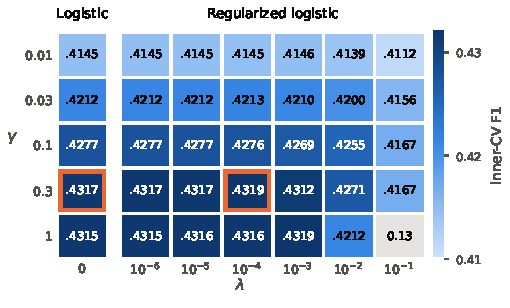
\includegraphics[width=\columnwidth]{figures/tuning.pdf}
\caption{Inner-CV F1 on the full training set; $\lambda=0$: plain
logistic regression. F1 rises with $\gamma$ until gradient descent converges
and does not depend on $\lambda\le10^{-3}$. Orange: selected.}
\label{fig:tuning}
\end{figure}

\begin{table}[!h]
\centering\small
\setlength{\tabcolsep}{4pt}
\begin{tabular}{lccccc}
\toprule
Method & F1 & Prec. & Rec. & Acc. & Thr. \\
\midrule
GD (MSE) & \pending{} & & & & \\
SGD (MSE) & \pending{} & & & & \\
Least squares & \pending{} & & & & \\
Ridge & \pending{} & & & & \\
Logistic & 0.431 $\pm$ 0.005 & 0.359 & 0.540 & 0.874 & 0.20 \\
Reg.\ logistic & 0.432 $\pm$ 0.005 & 0.358 & 0.543 & 0.874 & 0.20 \\
\textbf{Final model} & \textbf{0.441 $\pm$ 0.006} & 0.369 & 0.549 & 0.877 & 0.21 \\
\bottomrule
\end{tabular}
\caption{Nested cross-validation, mean over the 5 test folds. Thr.: mean
selected threshold. All rows but the last one-hot encode the nominal
features only. Always predicting ``no disease'' gives accuracy $0.912$ but
F1 $=0$.}
\label{tab:methods}
\end{table}

\begin{table}[!h]
\centering\small
\begin{tabular}{lcc}
\toprule
Configuration & F1 & $\Delta$ \\
\midrule
Generic baseline & 0.416 $\pm$ 0.005 & \\
+ codebook rules & 0.429 $\pm$ 0.003 & $+0.013\pm0.004$ \\
+ one-hot encoding & 0.433 $\pm$ 0.005 & $+0.004\pm0.003$ \\
+ missing indicators & 0.438 $\pm$ 0.004 & $+0.005\pm0.002$ \\
+ 40-feature interactions & 0.441 $\pm$ 0.006 & $+0.003\pm0.002$ \\
\bottomrule
\end{tabular}
\caption{From the baseline to the final model, one change per row.
$\Delta$: per-fold gain over the row above. After the baseline,
$\gamma=0.3$ and $\lambda=10^{-4}$.}
\label{tab:ablation}
\end{table}

The gain therefore comes from the features, which Table~\ref{tab:ablation}
adds one at a time. The codebook rules contribute most, through precision,
which rises from $0.337$ to $0.361$. One-hot encoding and missing indicators
then add $0.004$ and $0.005$ in all folds, and the interactions $0.003$ in
four folds only, a likely but not certain gain. Other additions, such as
squared or binned features, more interactions or model averaging, changed
F1 by less than $0.001$.

Finally, the class imbalance needs no correction beyond the threshold.
Multiplying the loss of the positive samples by $3.2$ or $10.3$, the ratio
of negatives to positives, barely changes F1, $0.431$ and $0.430$ against
$0.432$, but raises the selected threshold from $0.21$ to $0.48$ and $0.75$.
Weighting raises all predicted probabilities while keeping their order, so
a higher threshold gives back the same predictions: as the odds are
multiplied by about $\omega$, $0.21$ becomes $0.73$ for $\omega=10.3$.

% ============================================================================
% OWNER: Person 3 (conclusion, reproducibility)
% ============================================================================
\section{Conclusion}
The final model, regularized logistic regression with interactions, reaches
a nested-CV F1 of $0.441\pm0.006$ and $0.454$ on AIcrowd. The codebook rules
give the largest gain, the model does not overfit, so regularization does
not help, and threshold tuning already handles the imbalance. The labels are
self-reported and the survey is observational, so the model captures
associations, not causes, and with a precision of $0.37$ most predicted
positives are false alarms. The small, uncertain gain of the interactions
suggests that linear models are close to their limit on these features.

\section*{Reproducibility}
Code: \pending{public GitHub URL and commit}. \texttt{run.py} reproduces the
submitted predictions. \texttt{tune\_models.py}, \texttt{evaluate\_best.py}
and \texttt{imbalance.py} produce Tables~\ref{tab:methods}
and~\ref{tab:ablation}, and \texttt{plots.py} draws Fig.~\ref{fig:tuning};
the README lists all commands.

\bibliographystyle{IEEEtran}
\bibliography{references}

\end{document}
